% !TEX program = xelatex

\documentclass{article}
\usepackage{xeCJK}
\setmainfont[Path=fonts/, BoldFont=*-Bold, UprightFont=*-regular, ItalicFont=*-It]{MinionPro}
\setCJKmainfont[Path=fonts/]{BabelStoneHanFAE0.ttf}
\usepackage[vmargin=1in,hmargin=0.3in]{geometry}
\usepackage{fancyhdr}
\pagestyle{fancy}
\fancyhf{}
\rhead{ISO/IEC JTC1/SC2/WG2/IRG N2511}
\lhead{Universal Multiple-Octet Coded Character Set}
\cfoot{\thepage}
\usepackage{caption}
\usepackage{hyperref}
\usepackage{graphicx}
\graphicspath{{./images/}}
\usepackage{cite}
\begin{document}

\begin{tabular}{l l}
Doc Type: & Working Group Document \\

Title: & Glyph issue for U+30759 \\

Source: & Huáng Jùnliàng (黃俊亮)  \\

Status: & Individual contribution \\

Action required: & To be considered by the IRG and UTC \\

Date: & \today \\
\end{tabular}

\section{Introduction}
The glyph of U+30759 appears to be unattested in multiple historical documents. We should either update the glyph or encode the correct form.

\section{Evidences}
Figure \ref{U30759} is the glyph at U+30759 in the current code chart, as of Unicode 13.0:
\begin{center}
    
\includegraphics{30759_U.pdf}
    \captionof{figure}{U+30759 ⽔ 85.14 UTC-01250}\label{U30759}
\end{center}

The evidence \footnote{Online Review Tool, \url{https://hc.jsecs.org/irg/ws2015/app/?id=02118}} of U+30759 comes from 《南明史》(2006年,中华书局)\cite[p. 1003]{南明史}.

The author 錢海岳 listed the references \cite[p. 5517]{南明史} including 《明實錄》 and 《明史稿》(萬斯同,抄本).

\newpage

However, 明史稿(萬斯同,抄本)\cite{明史稿萬斯同} gives {\huge 﫠} (⿱邦清) (Figure \ref{mingshigao}), although it seems 邦 and 清 are two separate characters, the writer is aware that 邦清 should combine into a single character, otherwise he should have shifted 嫡 to the next column.

\begin{center}
    \begin{tabular}{ c c }
        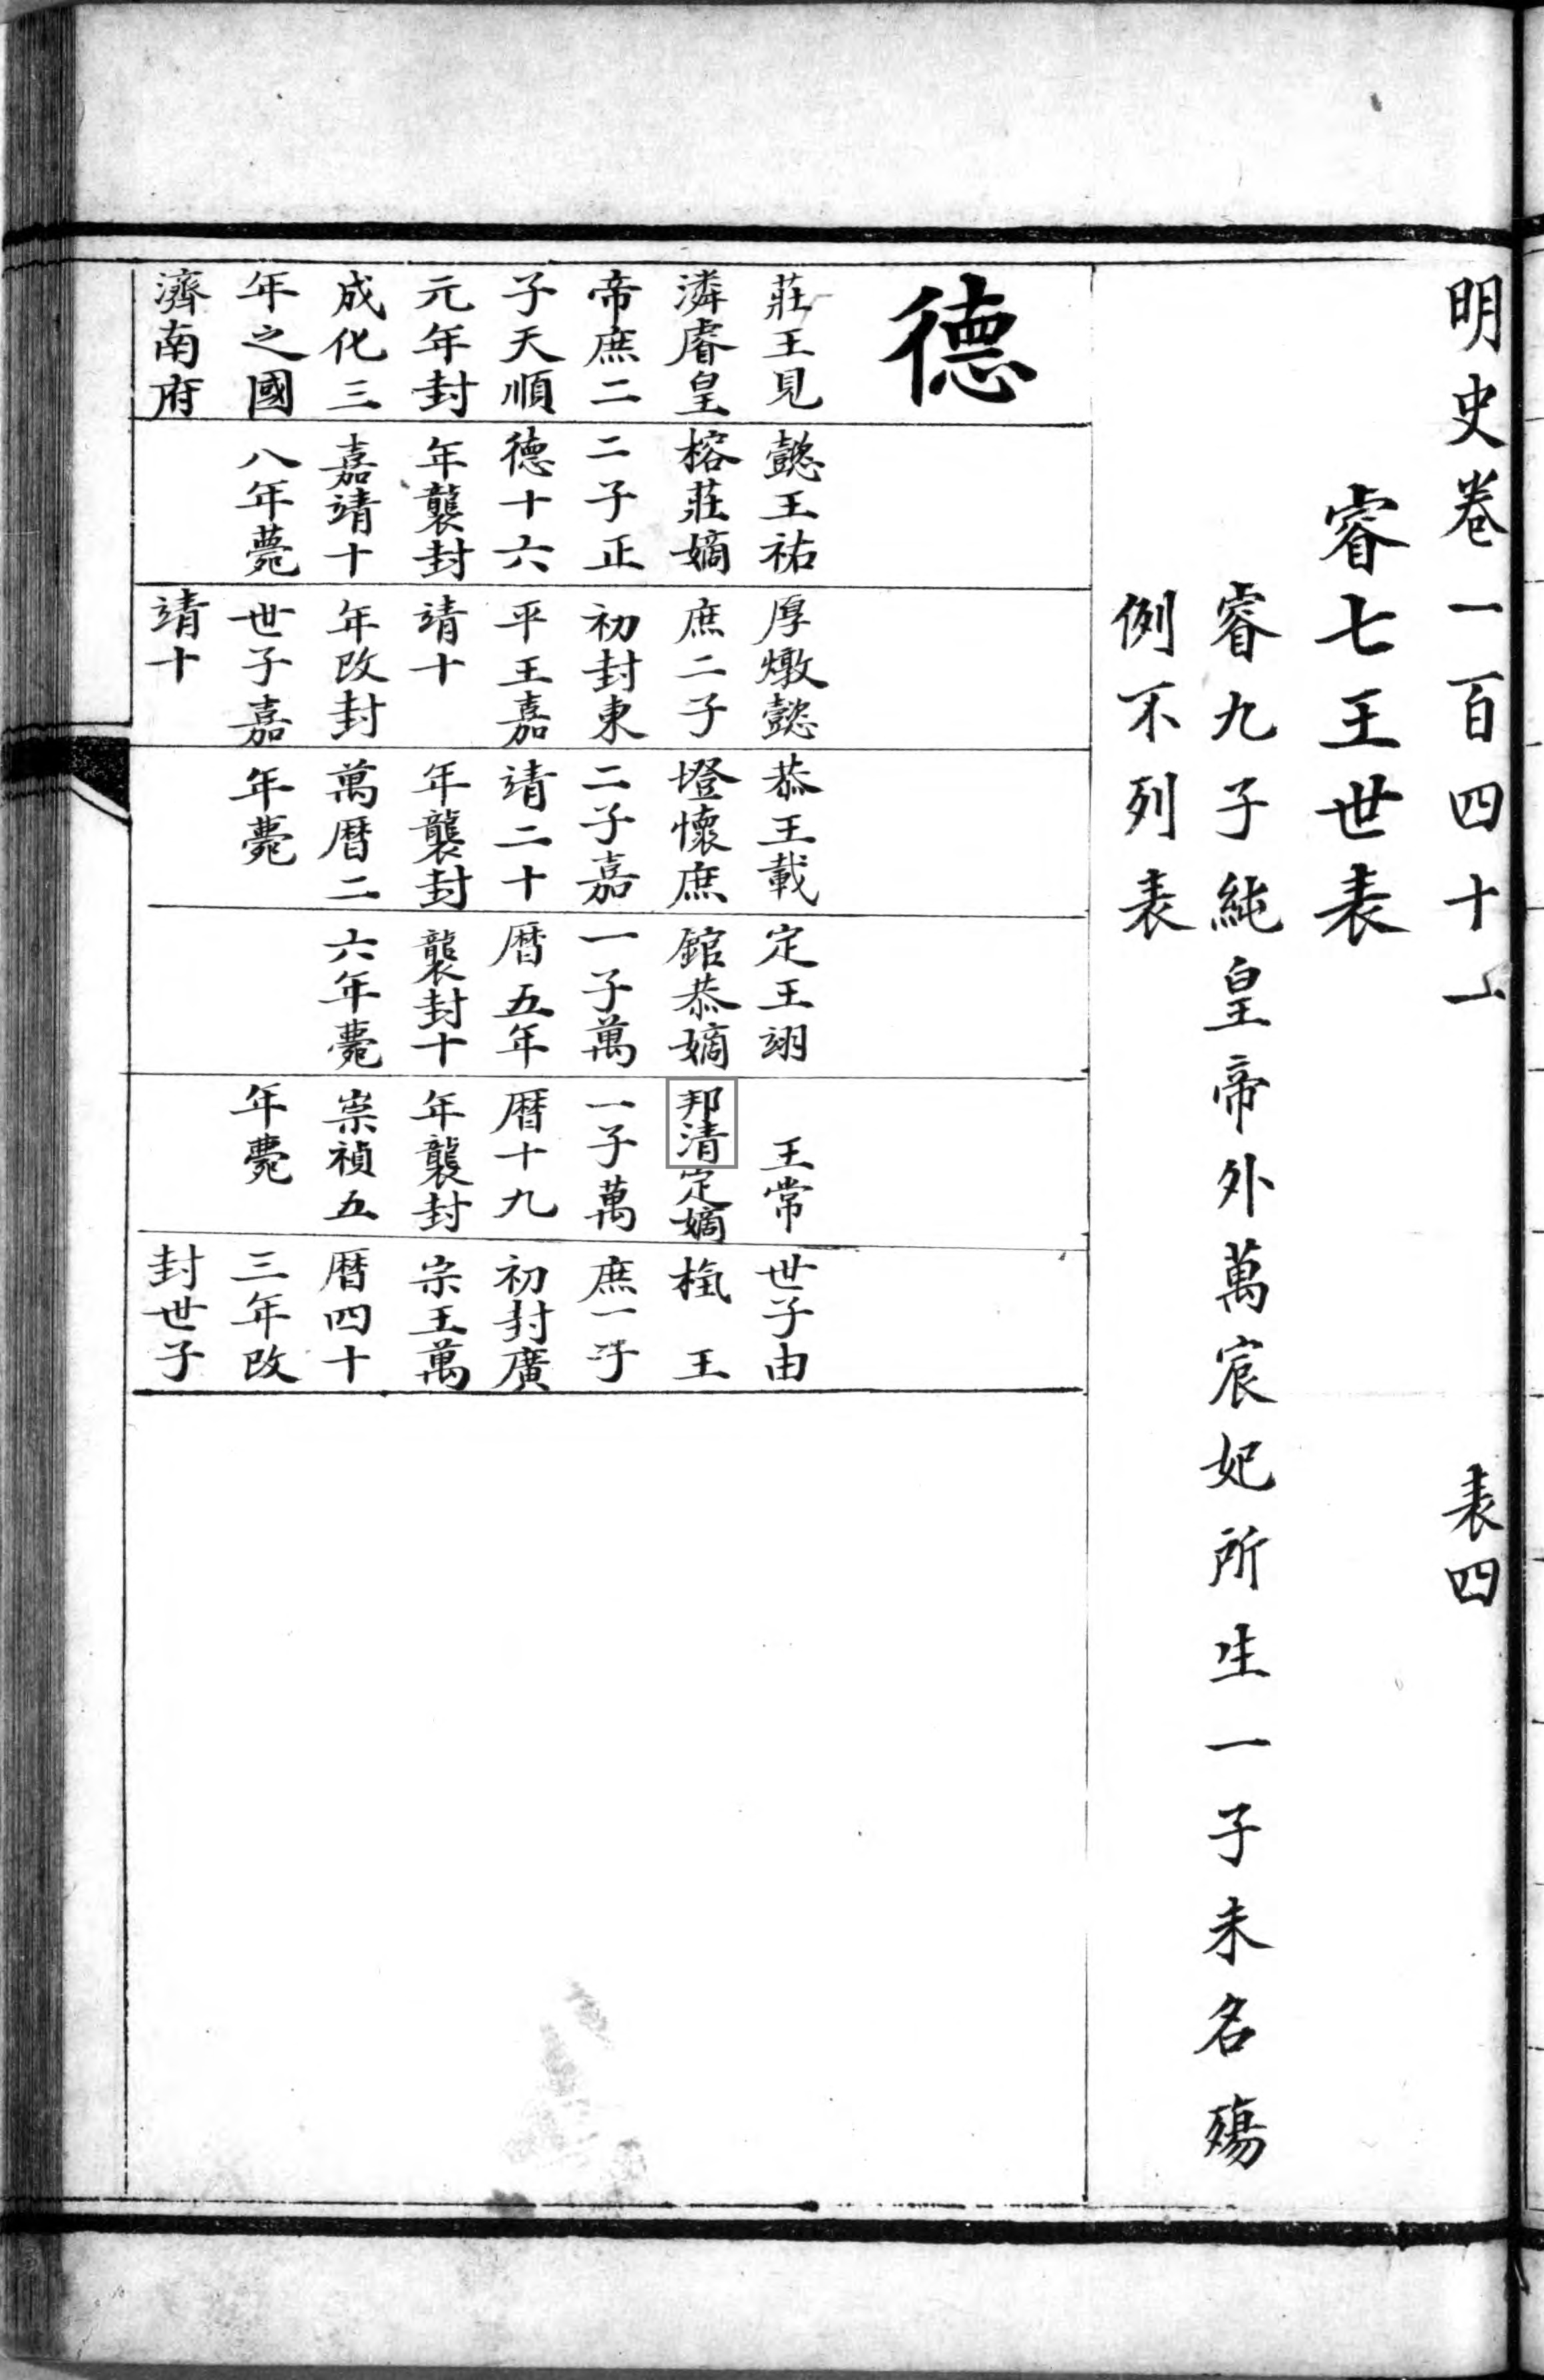
\includegraphics[height=.89\textheight]{95-0.jpg} & 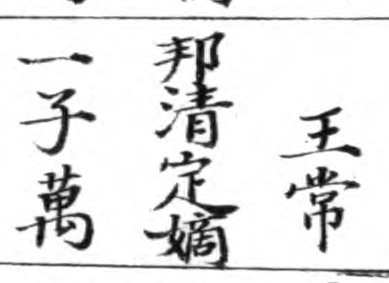
\includegraphics[width=.3\textwidth]{95-0-crop.png}
    \end{tabular}
    \captionof{figure}{明史稿(萬斯同,清抄本)卷141 folio 1}\label{mingshigao}
\end{center}

After 萬斯同 passed away, 王鴻緒 published 明史藁\cite{明史藁王鴻緖} in 1720. 明史藁 gives {\huge 﫢} (⿱邦󠄁淸) (Figure \ref{mingshigao1720}). Here 邦󠄁 is 邦 + VS18, a common variant of 邦; 淸 is unifiable to 清 under UCV \#319, so 﫢 can be unified to 﫠.

\begin{center}
    \begin{tabular}{ c c }
        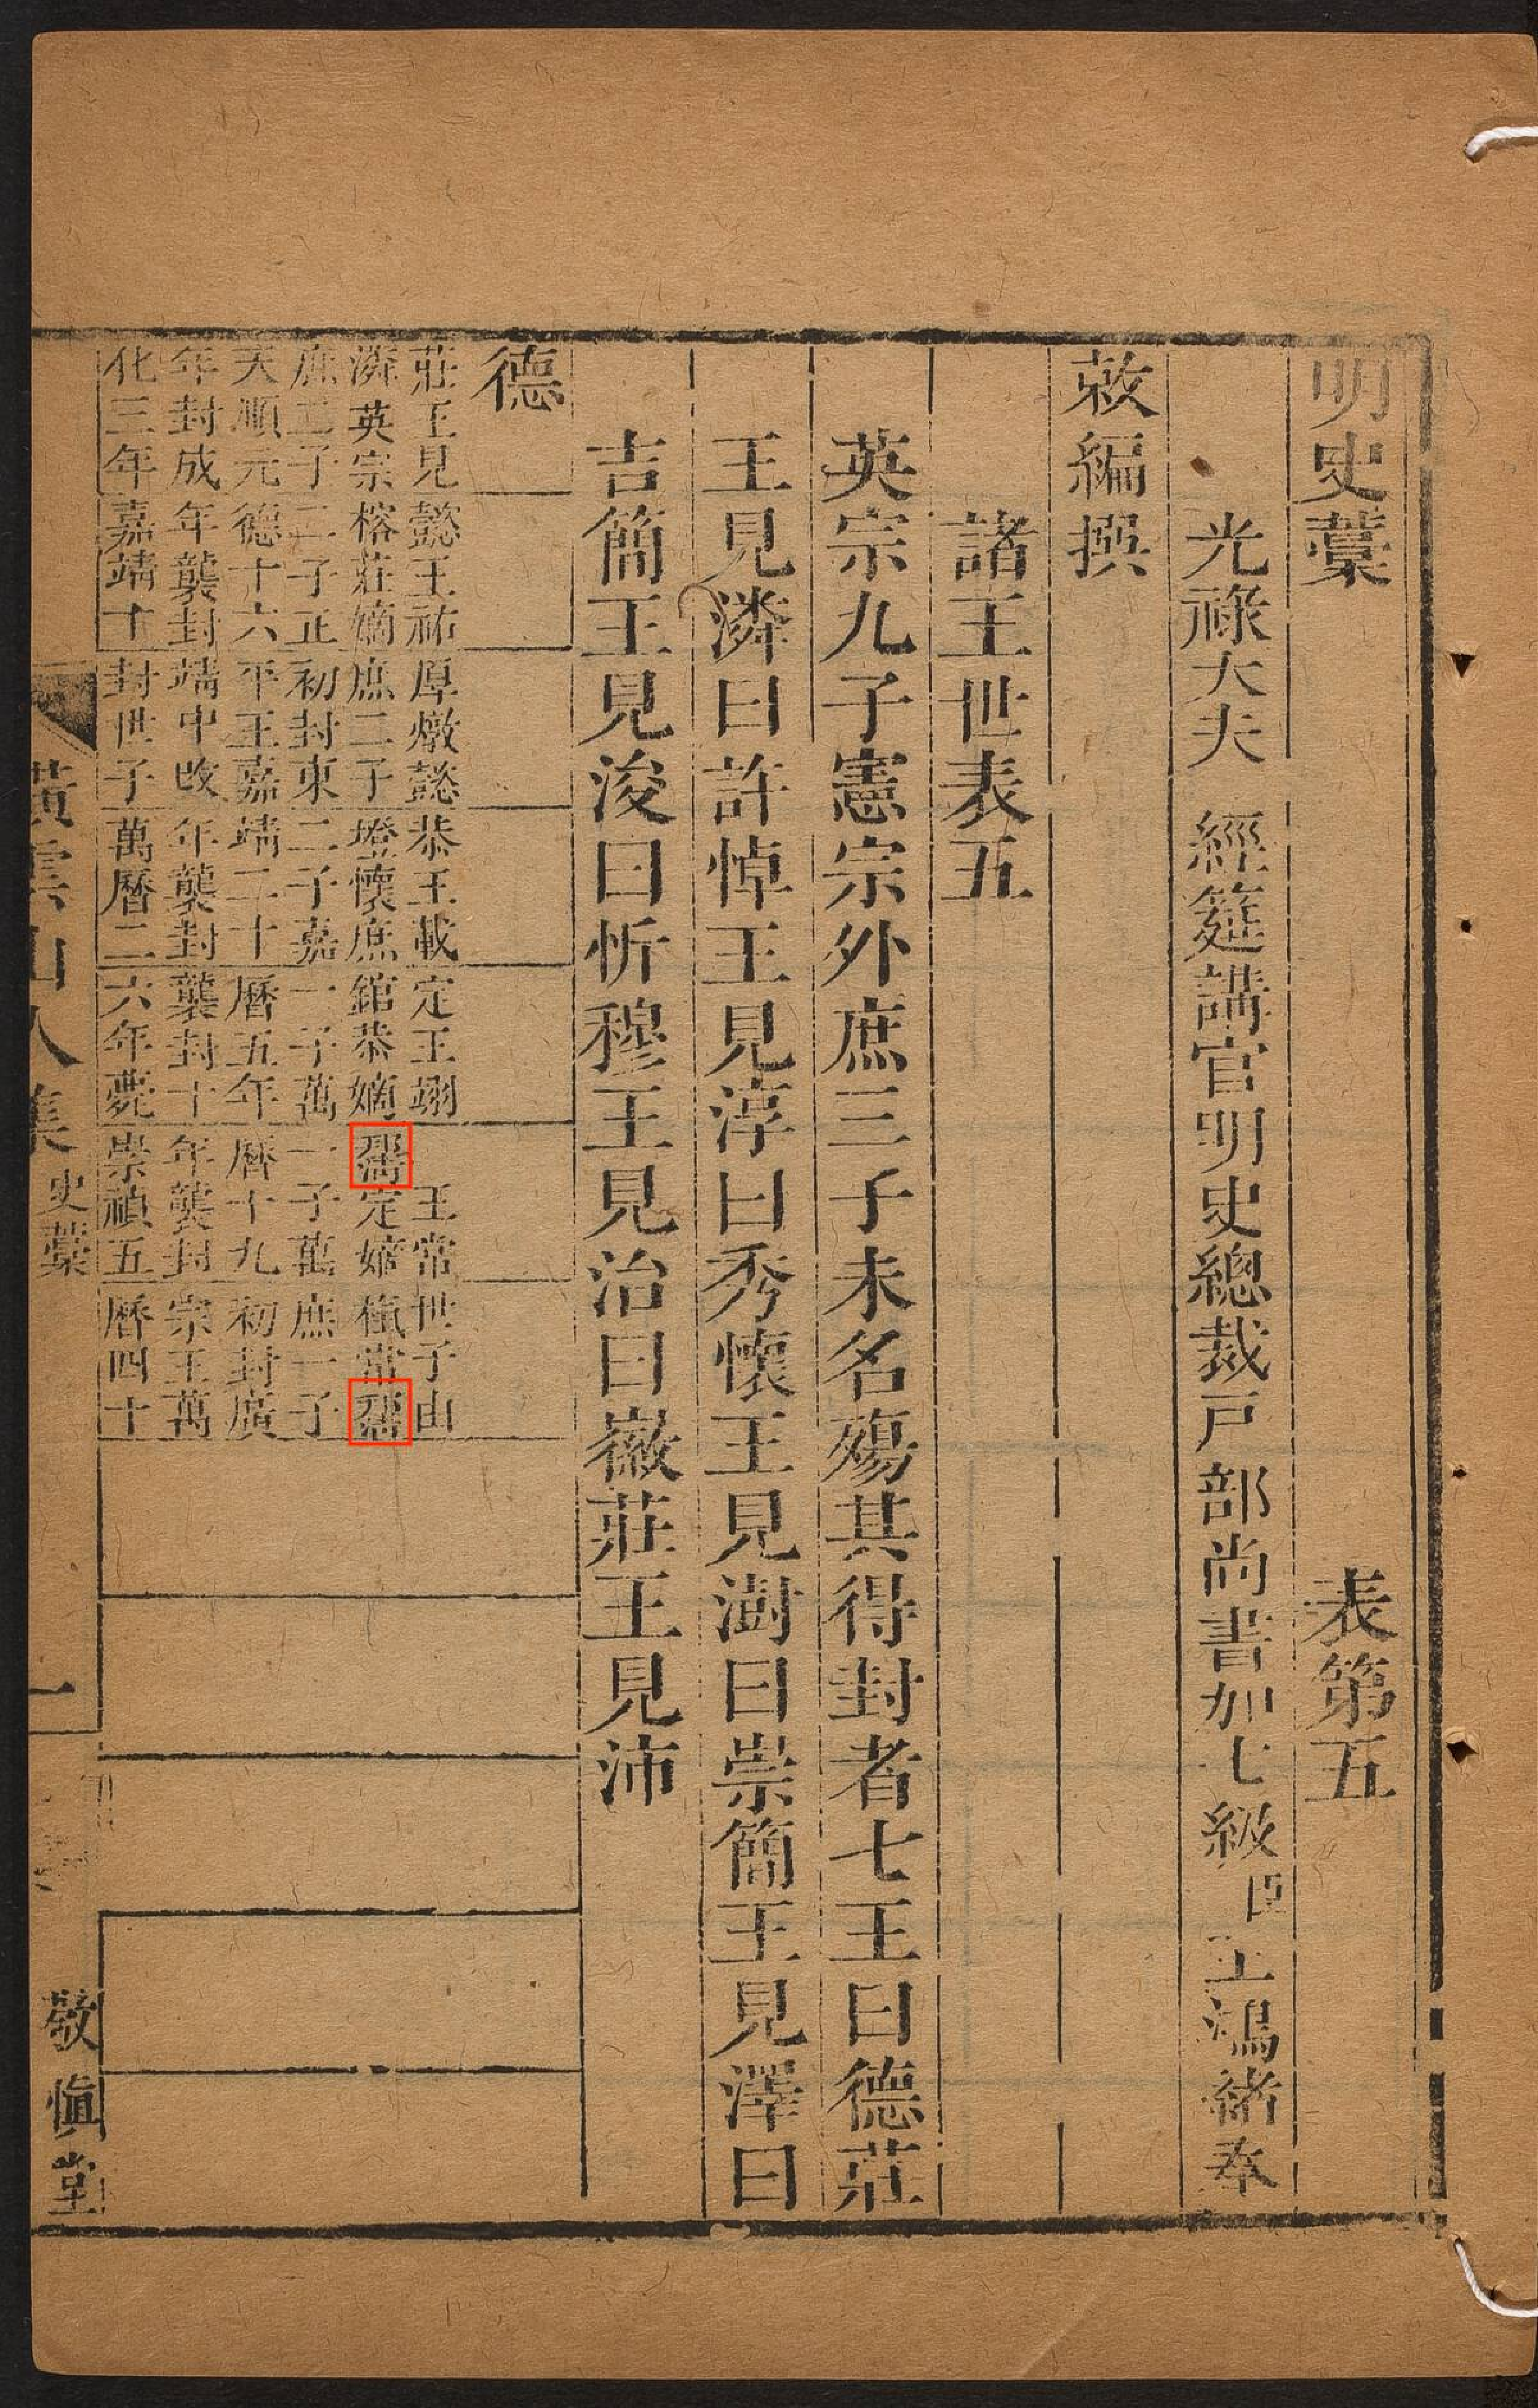
\includegraphics[height=.9\textheight]{24195504.png-0.pdf} & 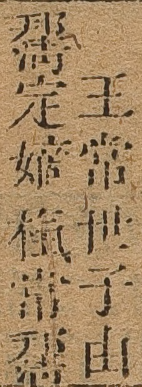
\includegraphics{24195504.png-0-crop.png}
    \end{tabular}
    \captionof{figure}{明史藁(王鴻緒,清雍正刊本)卷141 folio 1}\label{mingshigao1720}
\end{center}

明史 was then finalized in 武英殿 in 1739. 明史(武英殿本)\cite{明史武英殿}(Figure \ref{mingshi1739}) also gives {\huge 﫢} (⿱邦󠄁淸).

\begin{center}
    \begin{tabular}{ c c }
        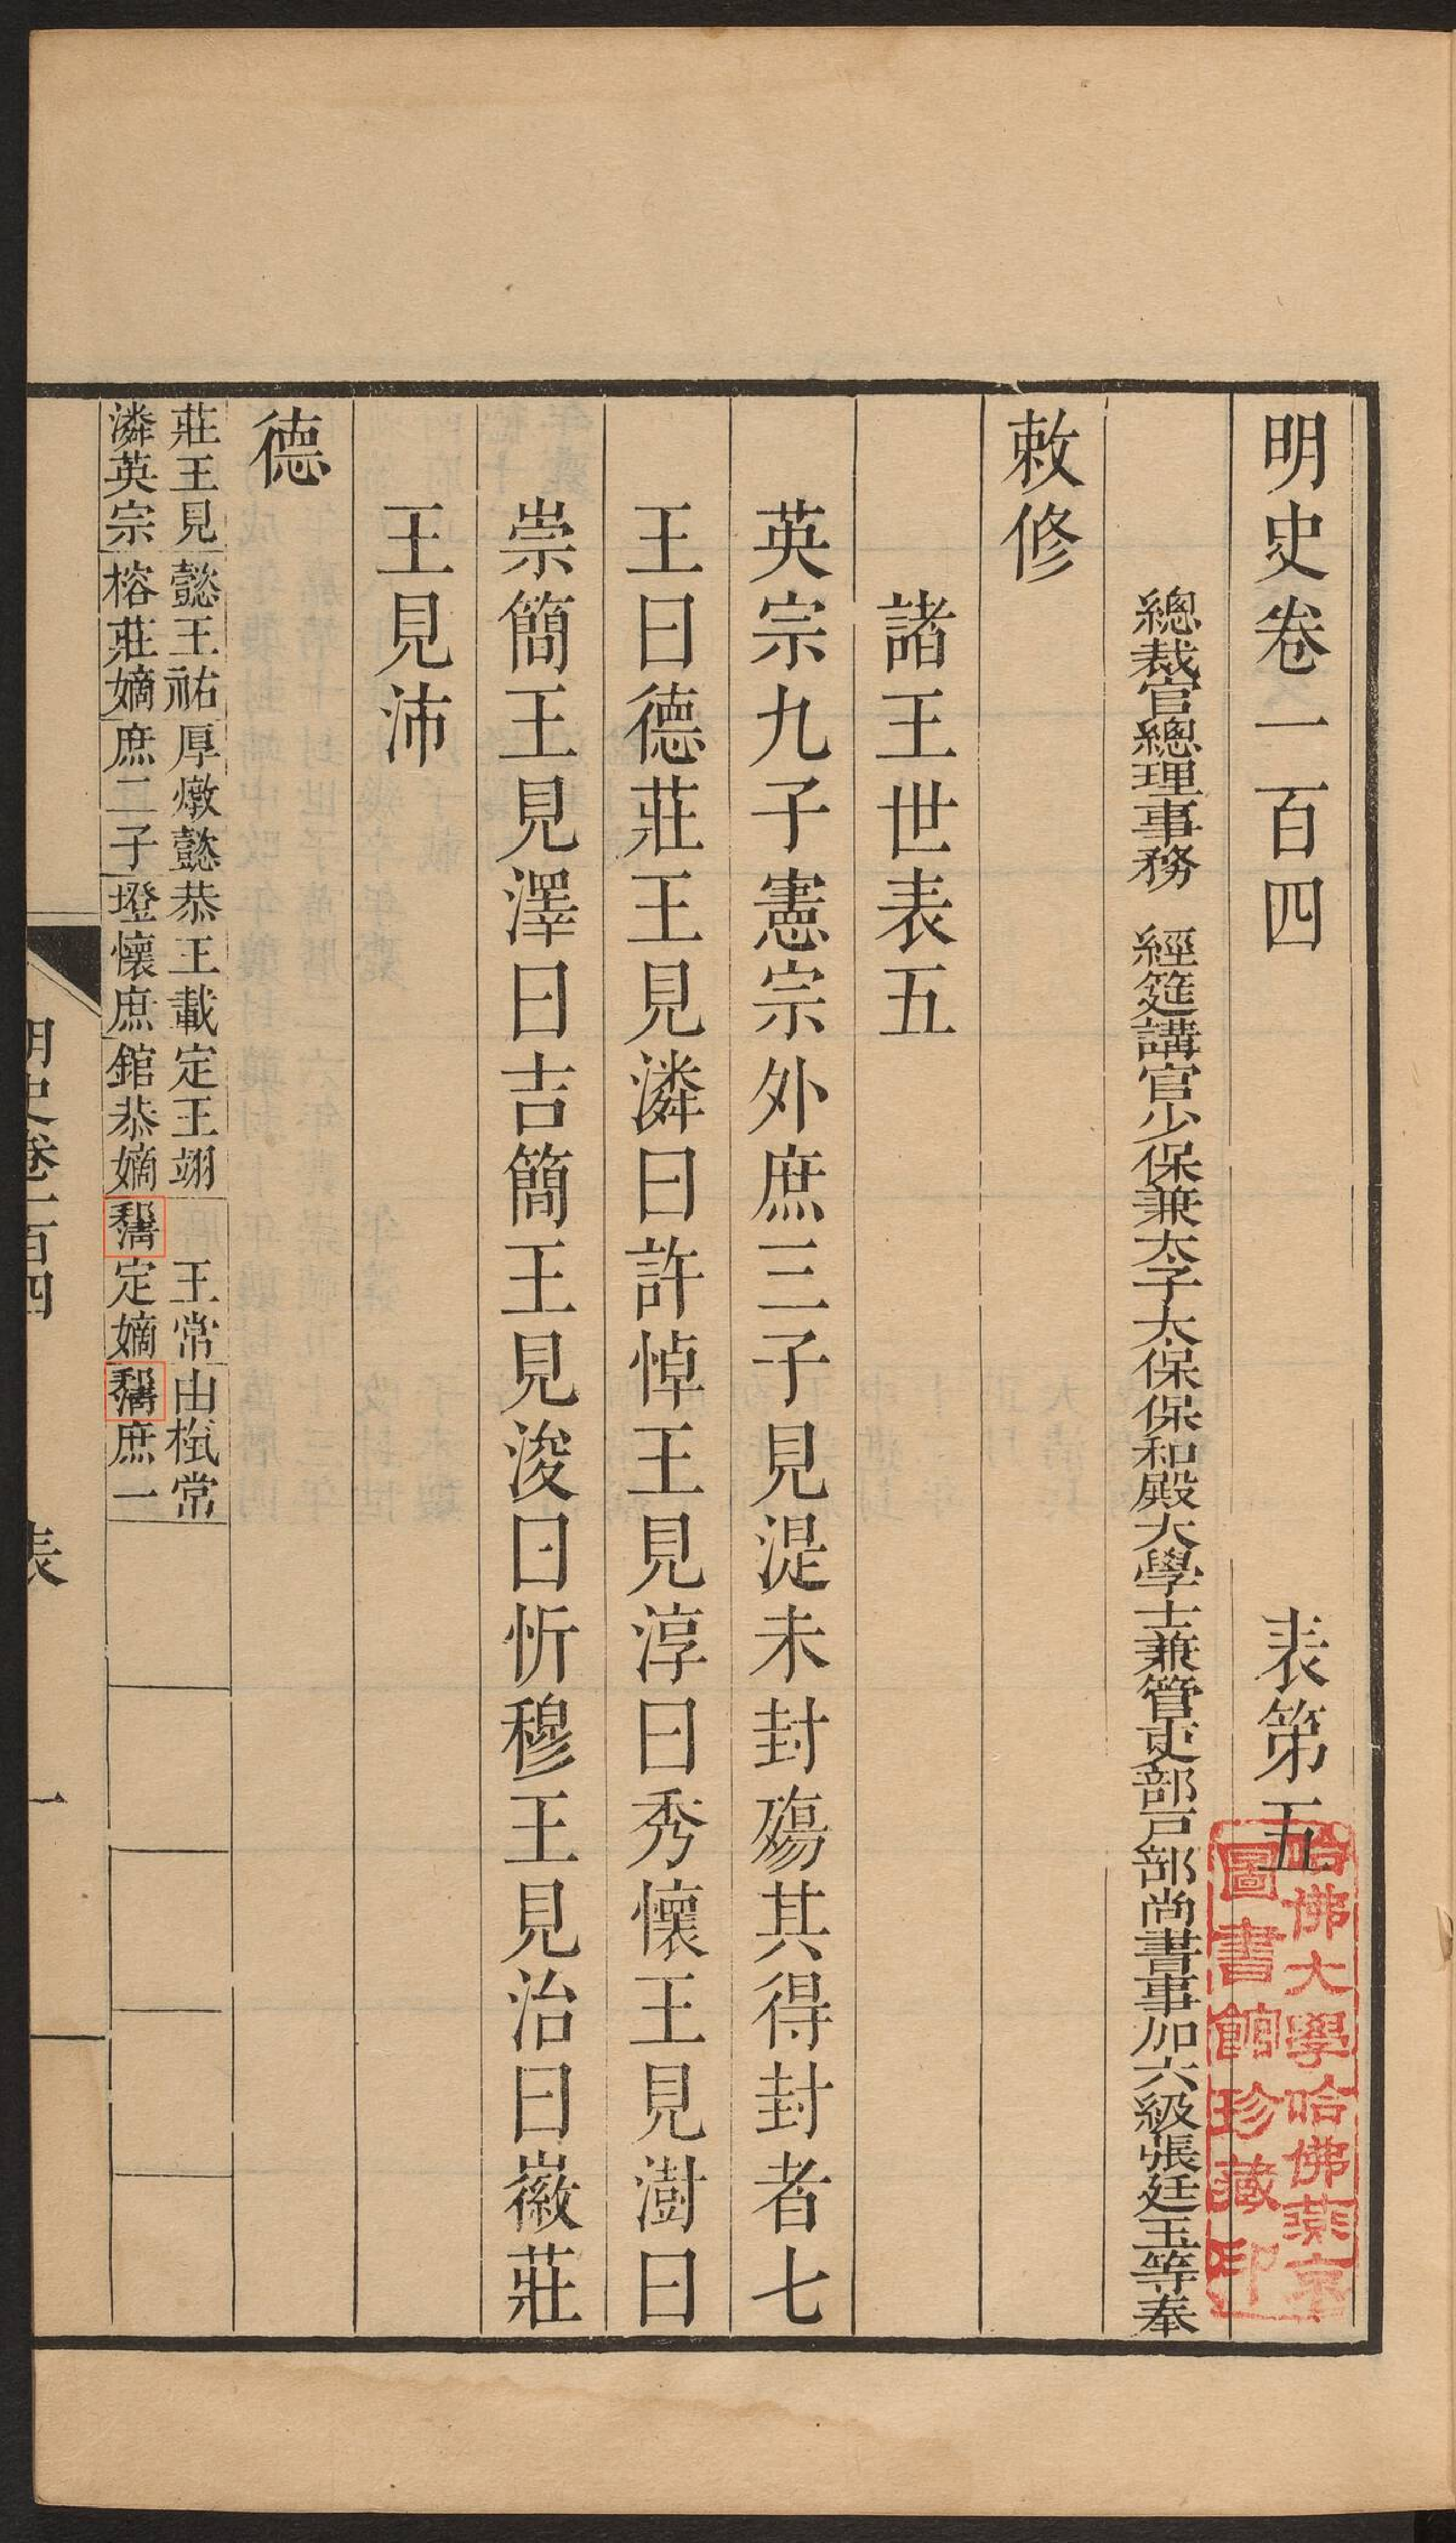
\includegraphics[height=.9\textheight]{24213151.png-0.pdf} & 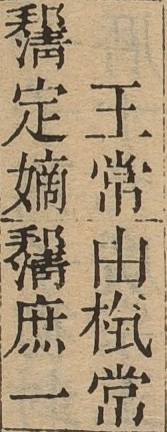
\includegraphics{24213151-crop.png}
    \end{tabular}
    \captionof{figure}{明史(清乾隆四年武英殿刊本)卷104 folio 1}\label{mingshi1739}
\end{center}

明實錄\cite{明實錄} (Figure \ref{mingshilu}) gives {\huge 﫡} (⿱邦󠄁清), which is also unifiable to 﫠.

\begin{center}
    \begin{tabular}{ c c }
        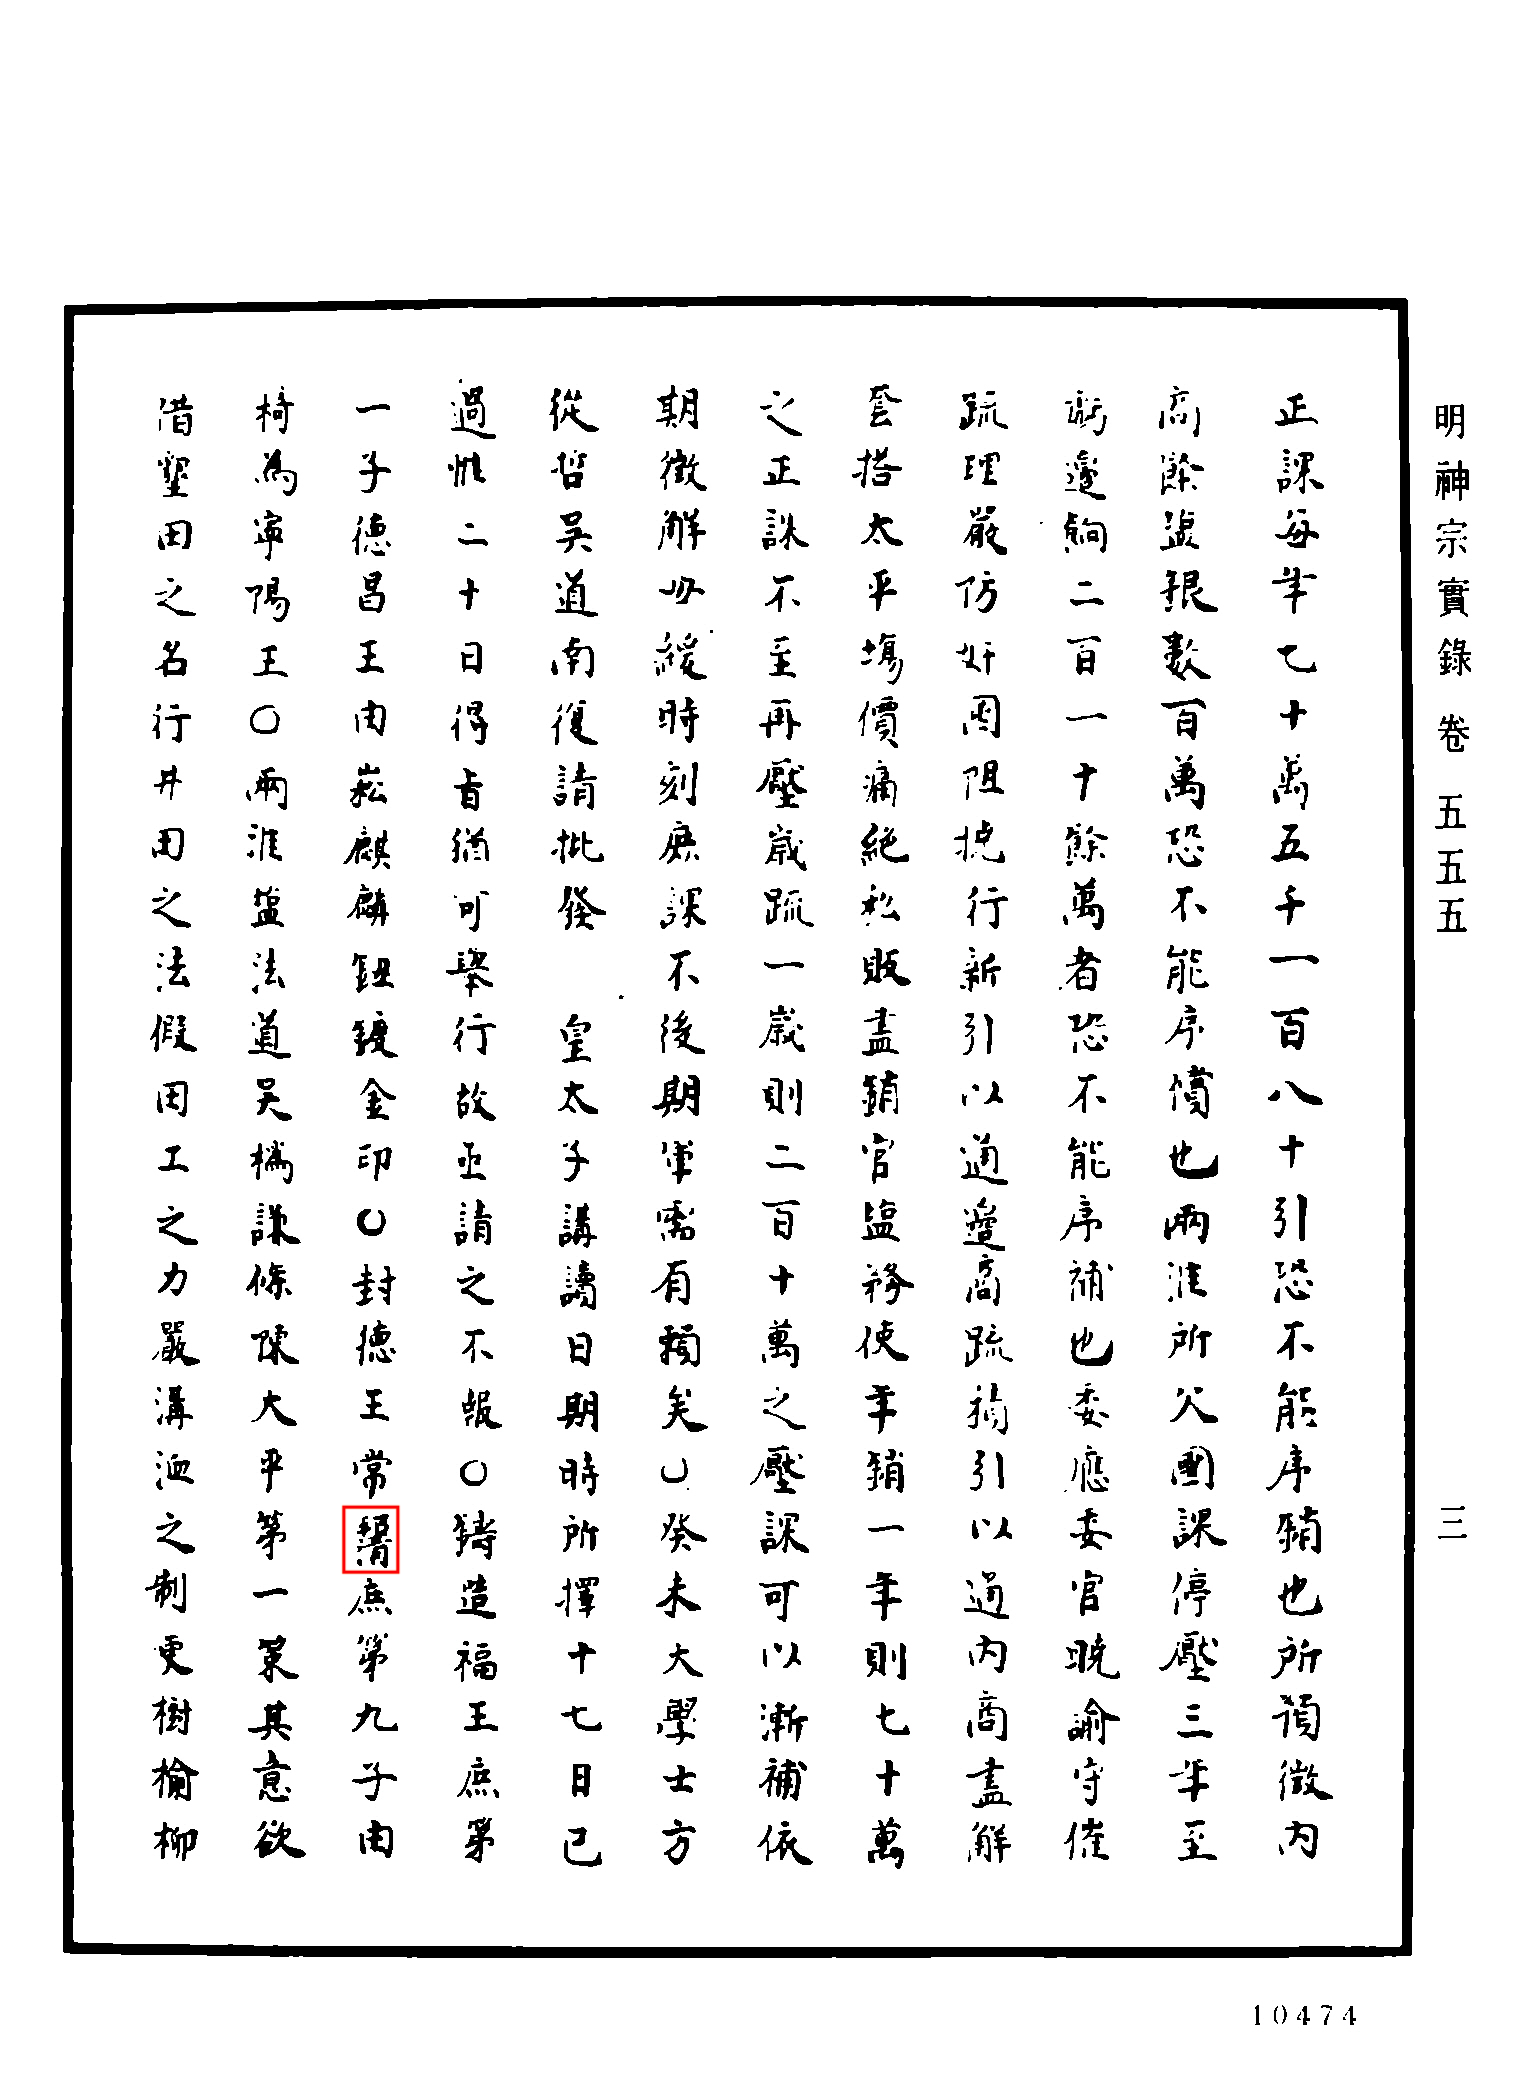
\includegraphics[height=.9\textheight]{msilok_0115550003b.png} & 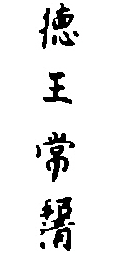
\includegraphics[scale=4]{msilok_0115550003b-crop.png}
    \end{tabular}
    \captionof{figure}{《明神宗實錄》(影印國立北平圖書館紅格鈔本)卷555 folio 3}\label{mingshilu}
\end{center}

The mentioned evidences were all created in Qīng dynasty. We can date back to 崇禎 era (1628-1644) when 朱常﫠 passed away, here 名山藏\cite{名山藏} gives {\huge 﫢} (⿱邦󠄁淸) (Figure \ref{mingshanzang}).

\begin{center}
    \begin{tabular}{ c c }
        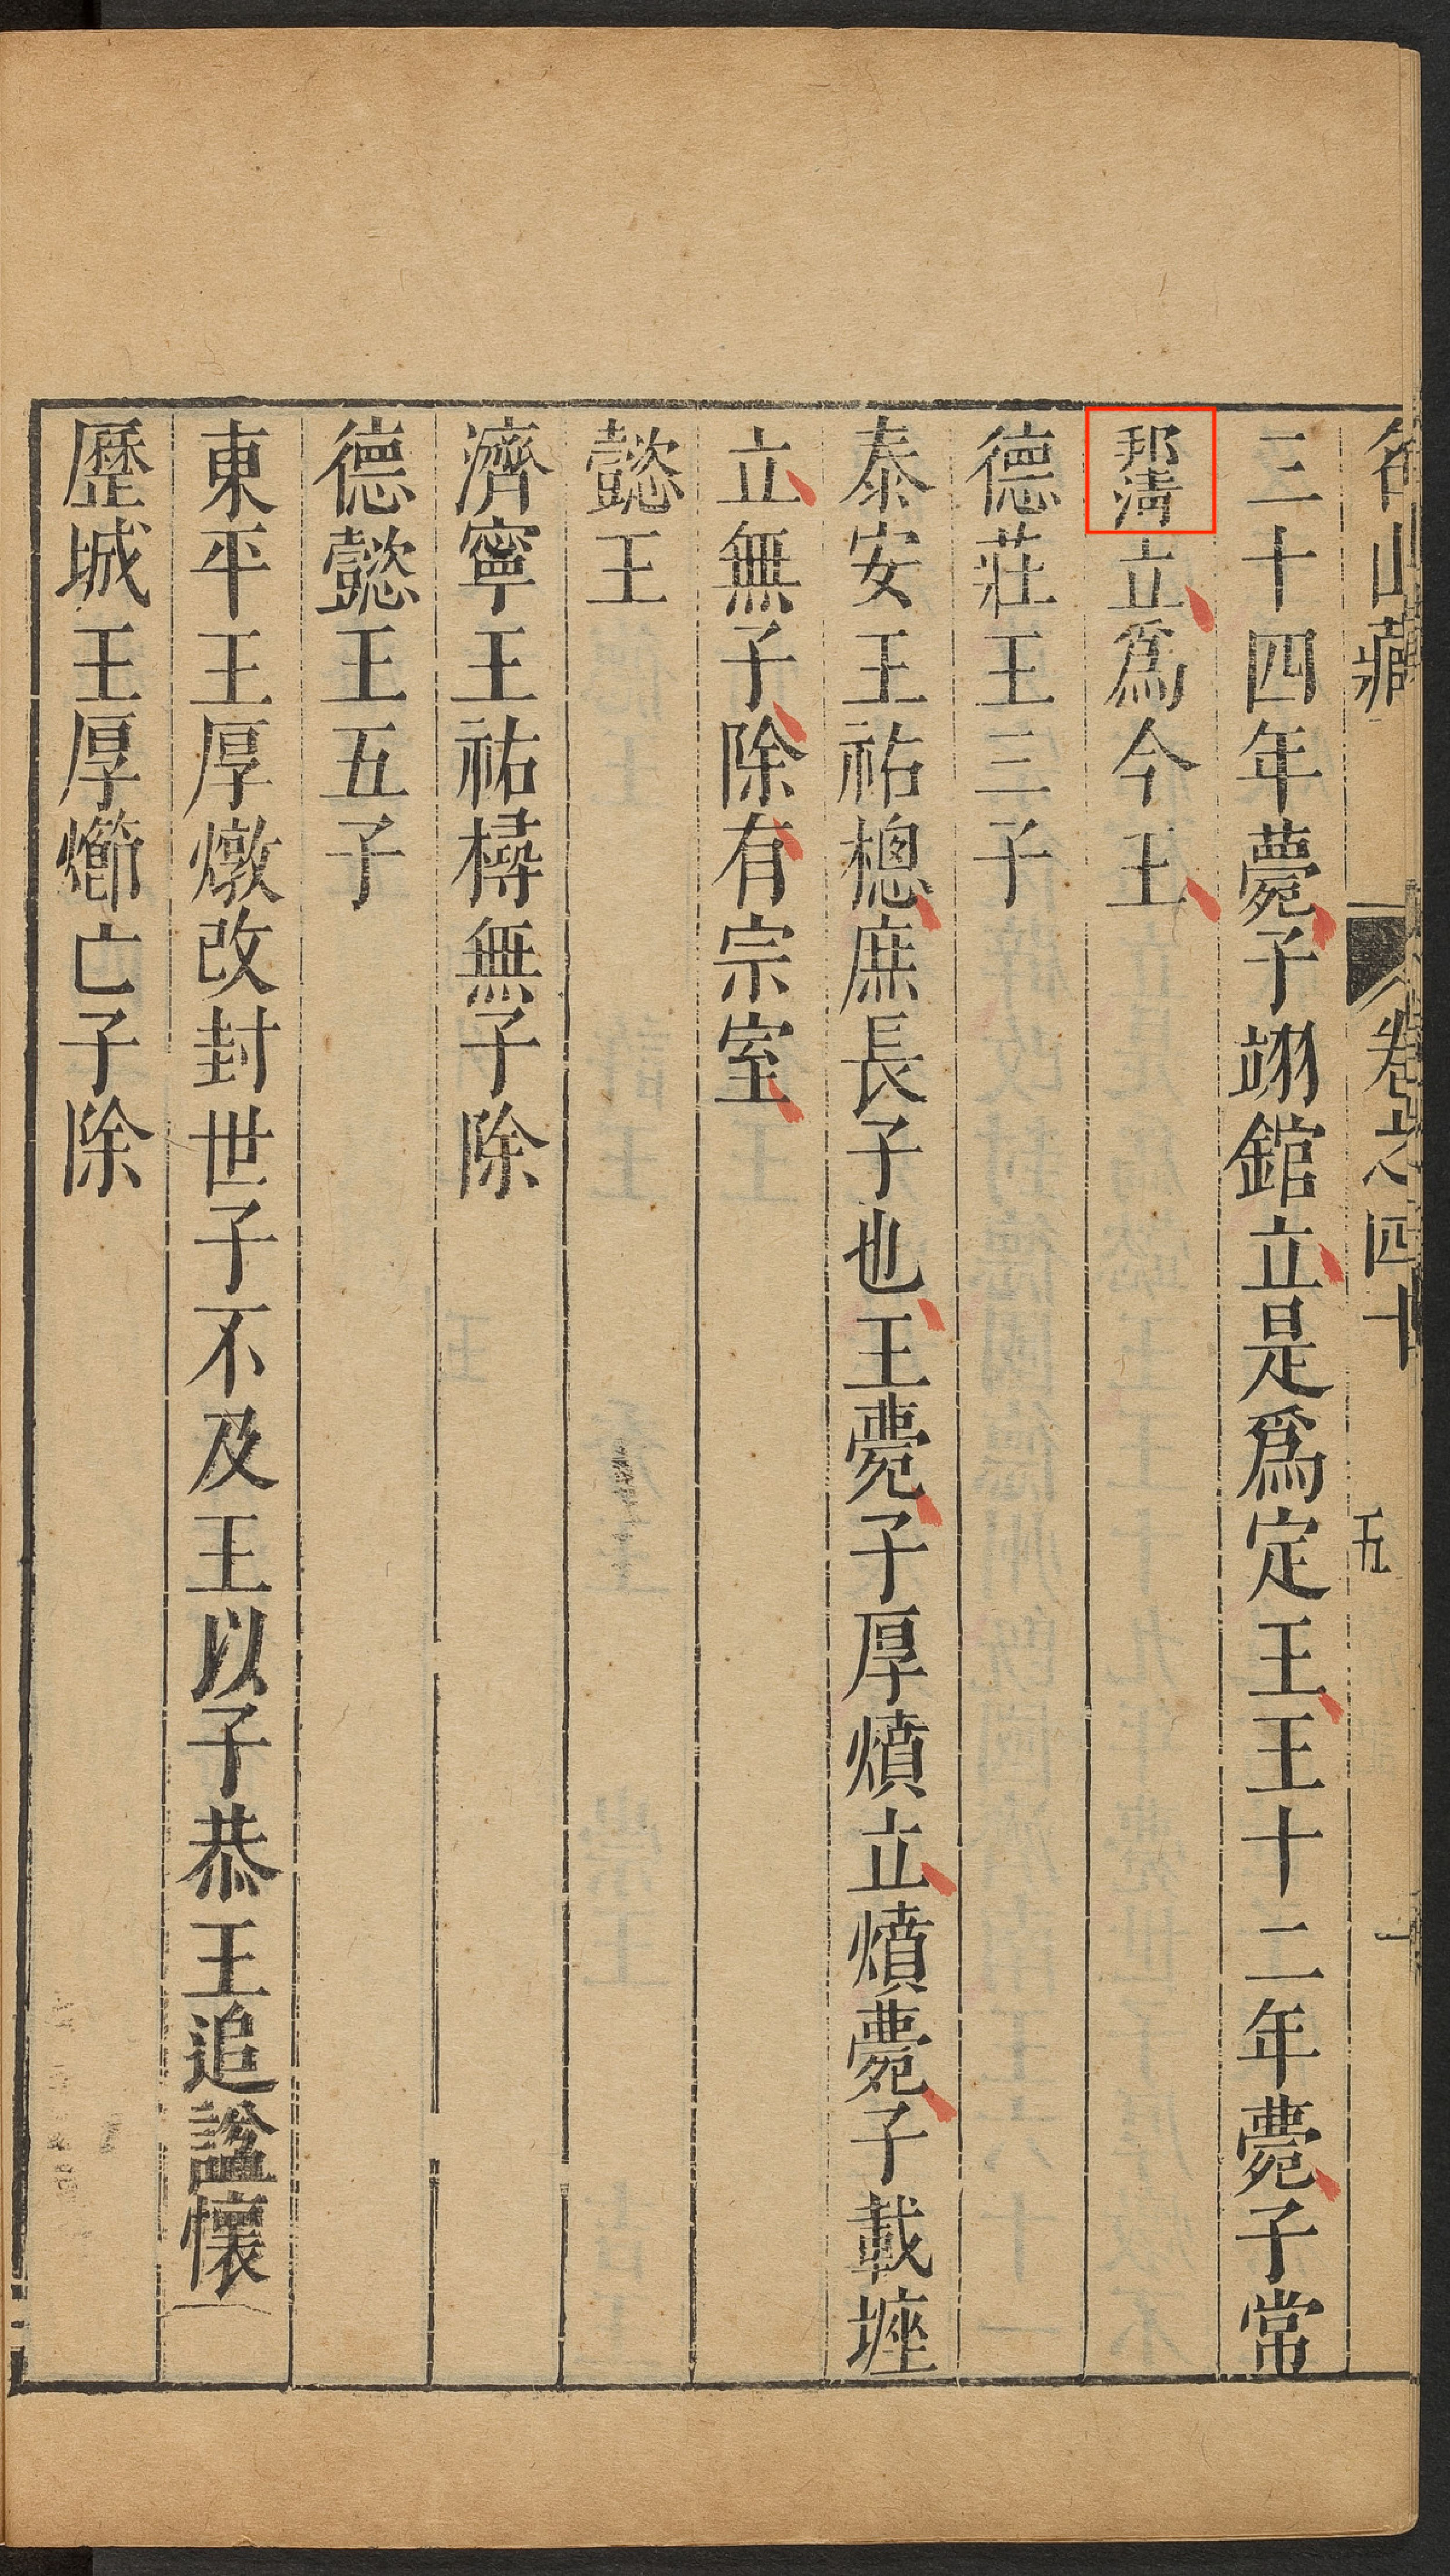
\includegraphics[height=.9\textheight]{20002484.png-1.pdf} & 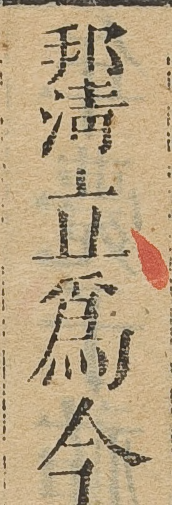
\includegraphics{20002484.png-1-crop.png}
    \end{tabular}
    \captionof{figure}{《名山藏》(明崇禎刊本)卷40 folio 1}\label{mingshanzang}
\end{center}

In 1939, 李晉華 published his last manuscripts 《明史德王府世系表訂誤》\cite{明史德王府世系表訂誤}, in which he had checked 德府玉牒 authored in 崇禎十一年 and corrected errors on the 德王's linearge table in 明史. The article gives 﫡, so we can assume 﫠 is also used in 德府玉牒.

\begin{center}
    \begin{tabular}{ c c }
        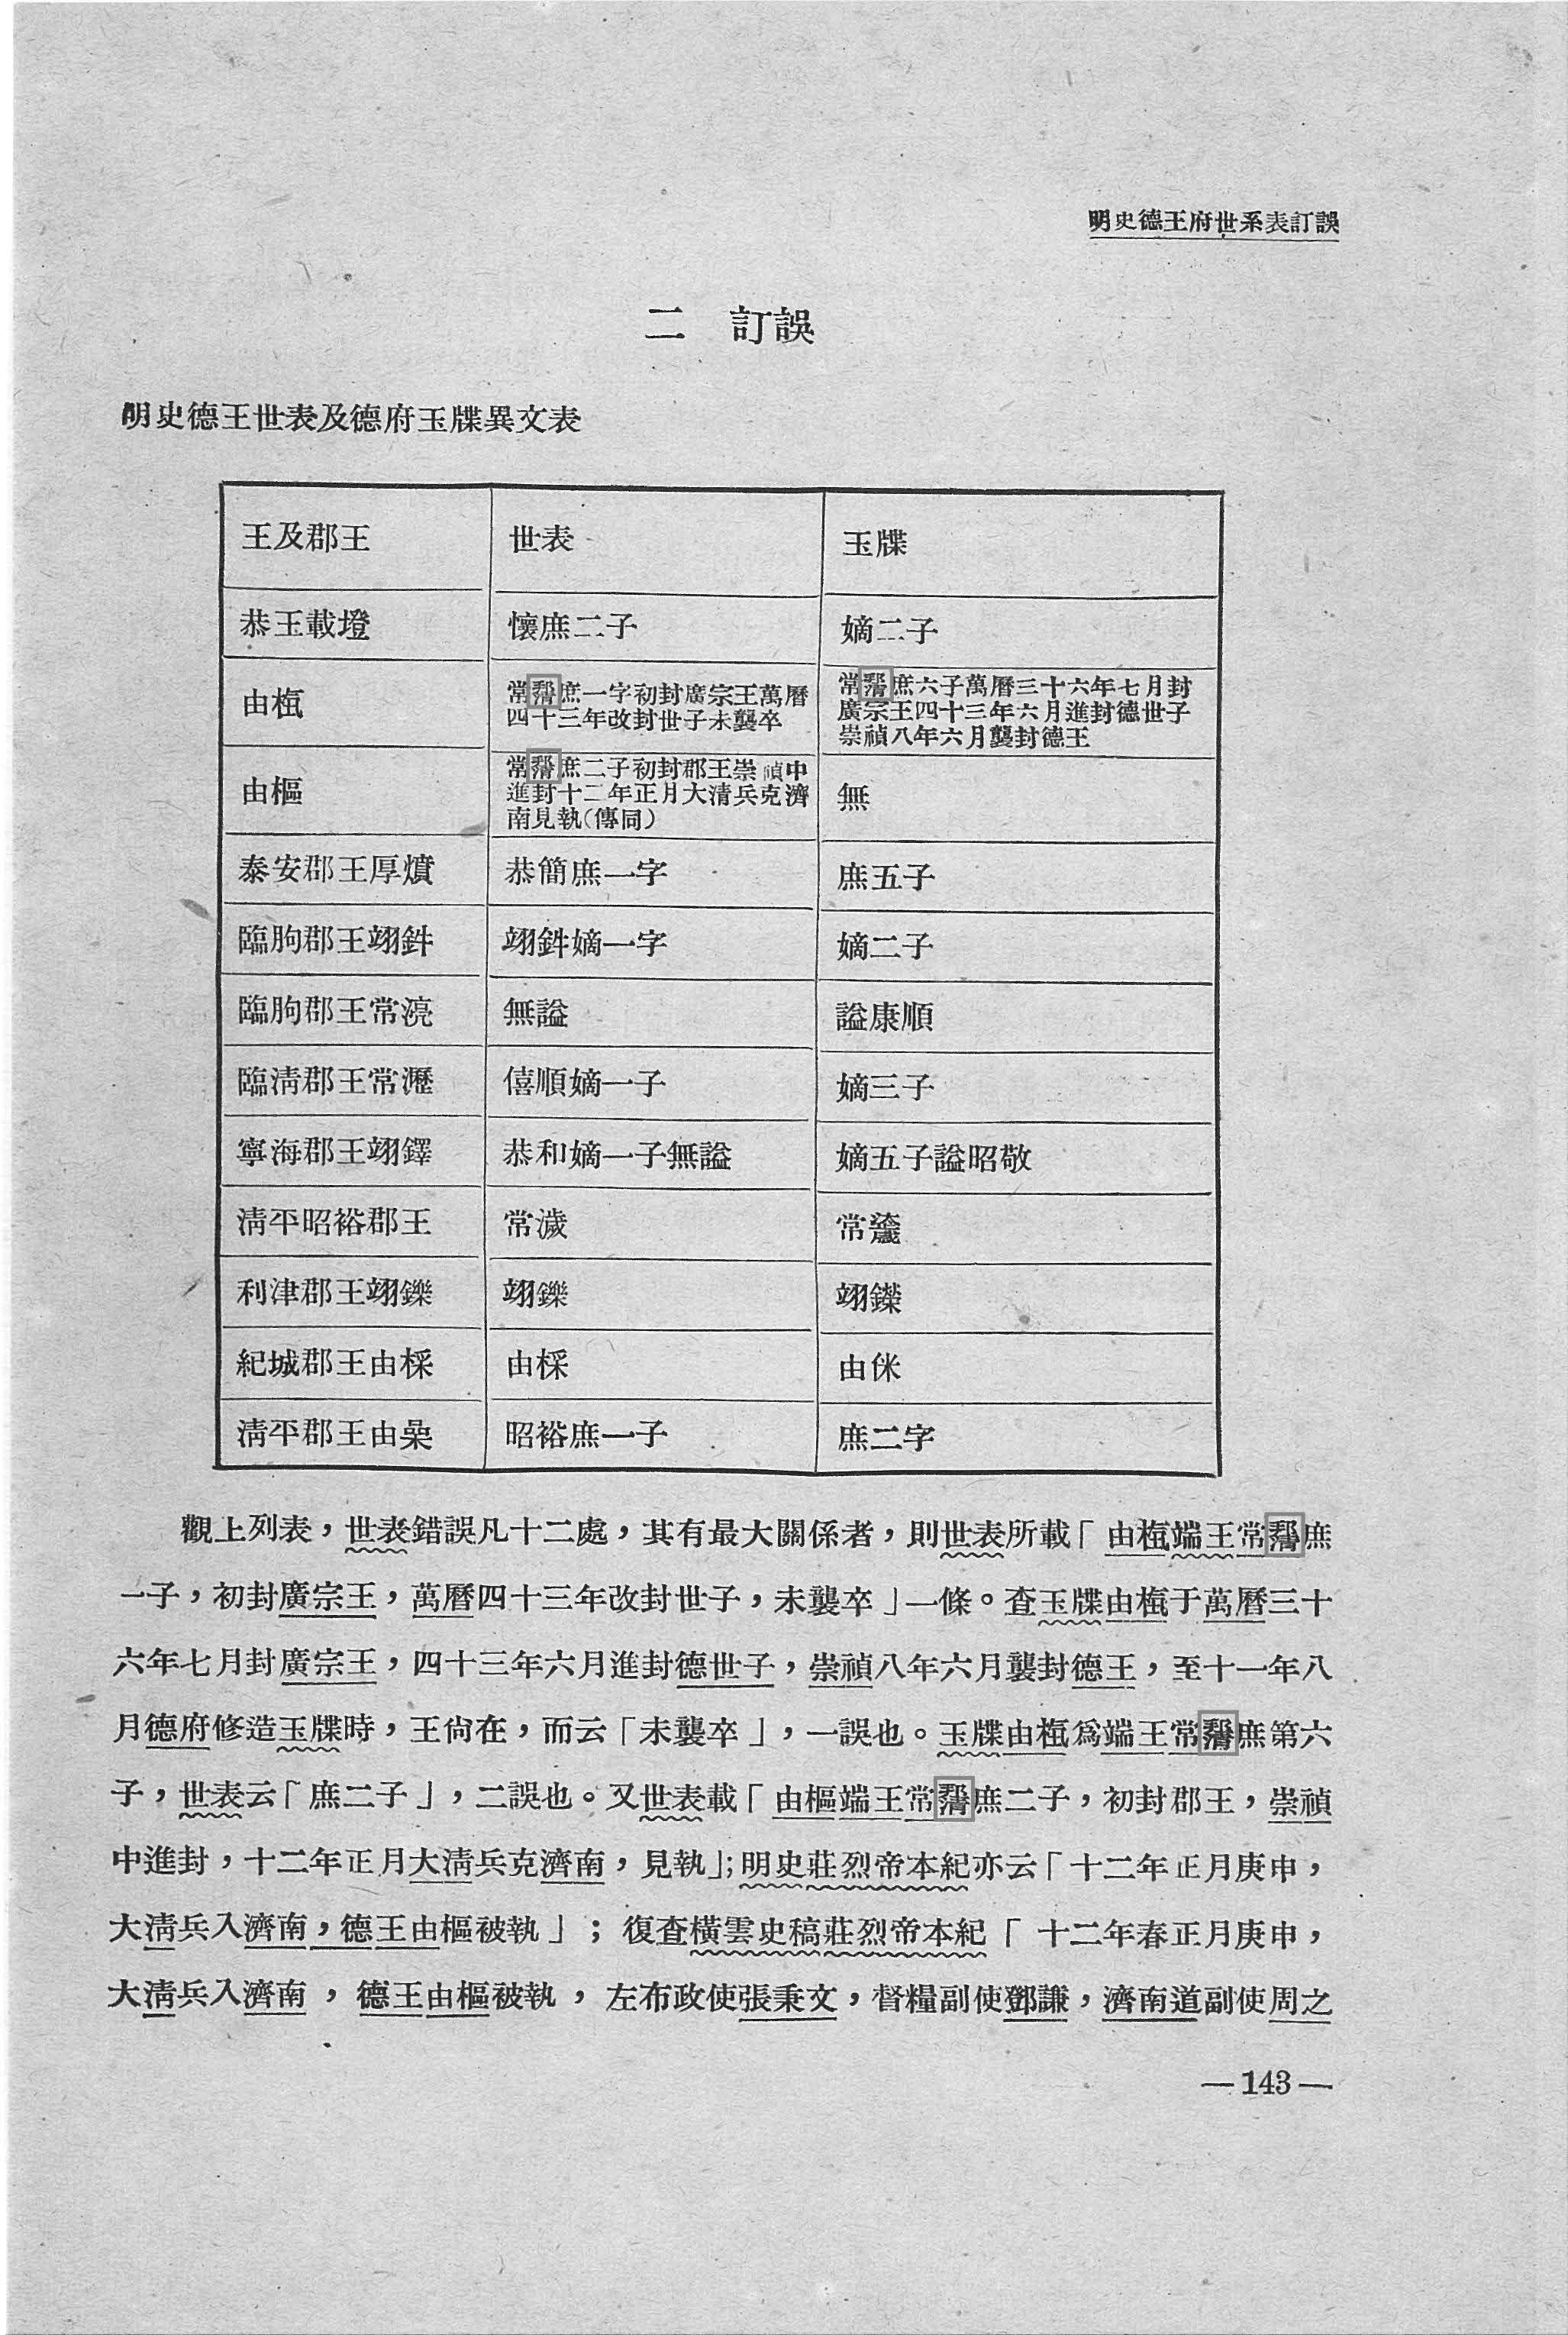
\includegraphics[height=.9\textheight]{5-000.jpg} & 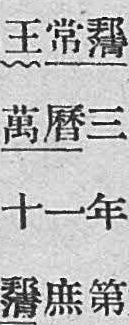
\includegraphics{5-000-crop.png}
    \end{tabular}
    \captionof{figure}{《明史德王府世系表訂誤》page 143}\label{mingshidewangfu}
\end{center}

\section{A modern evidence of 𰝙}

Interestingly, 明史(1974,中华书局)\cite[p. 2903]{明史1974} gives 𰝙.

\begin{center}
    \begin{tabular}{ c c }
        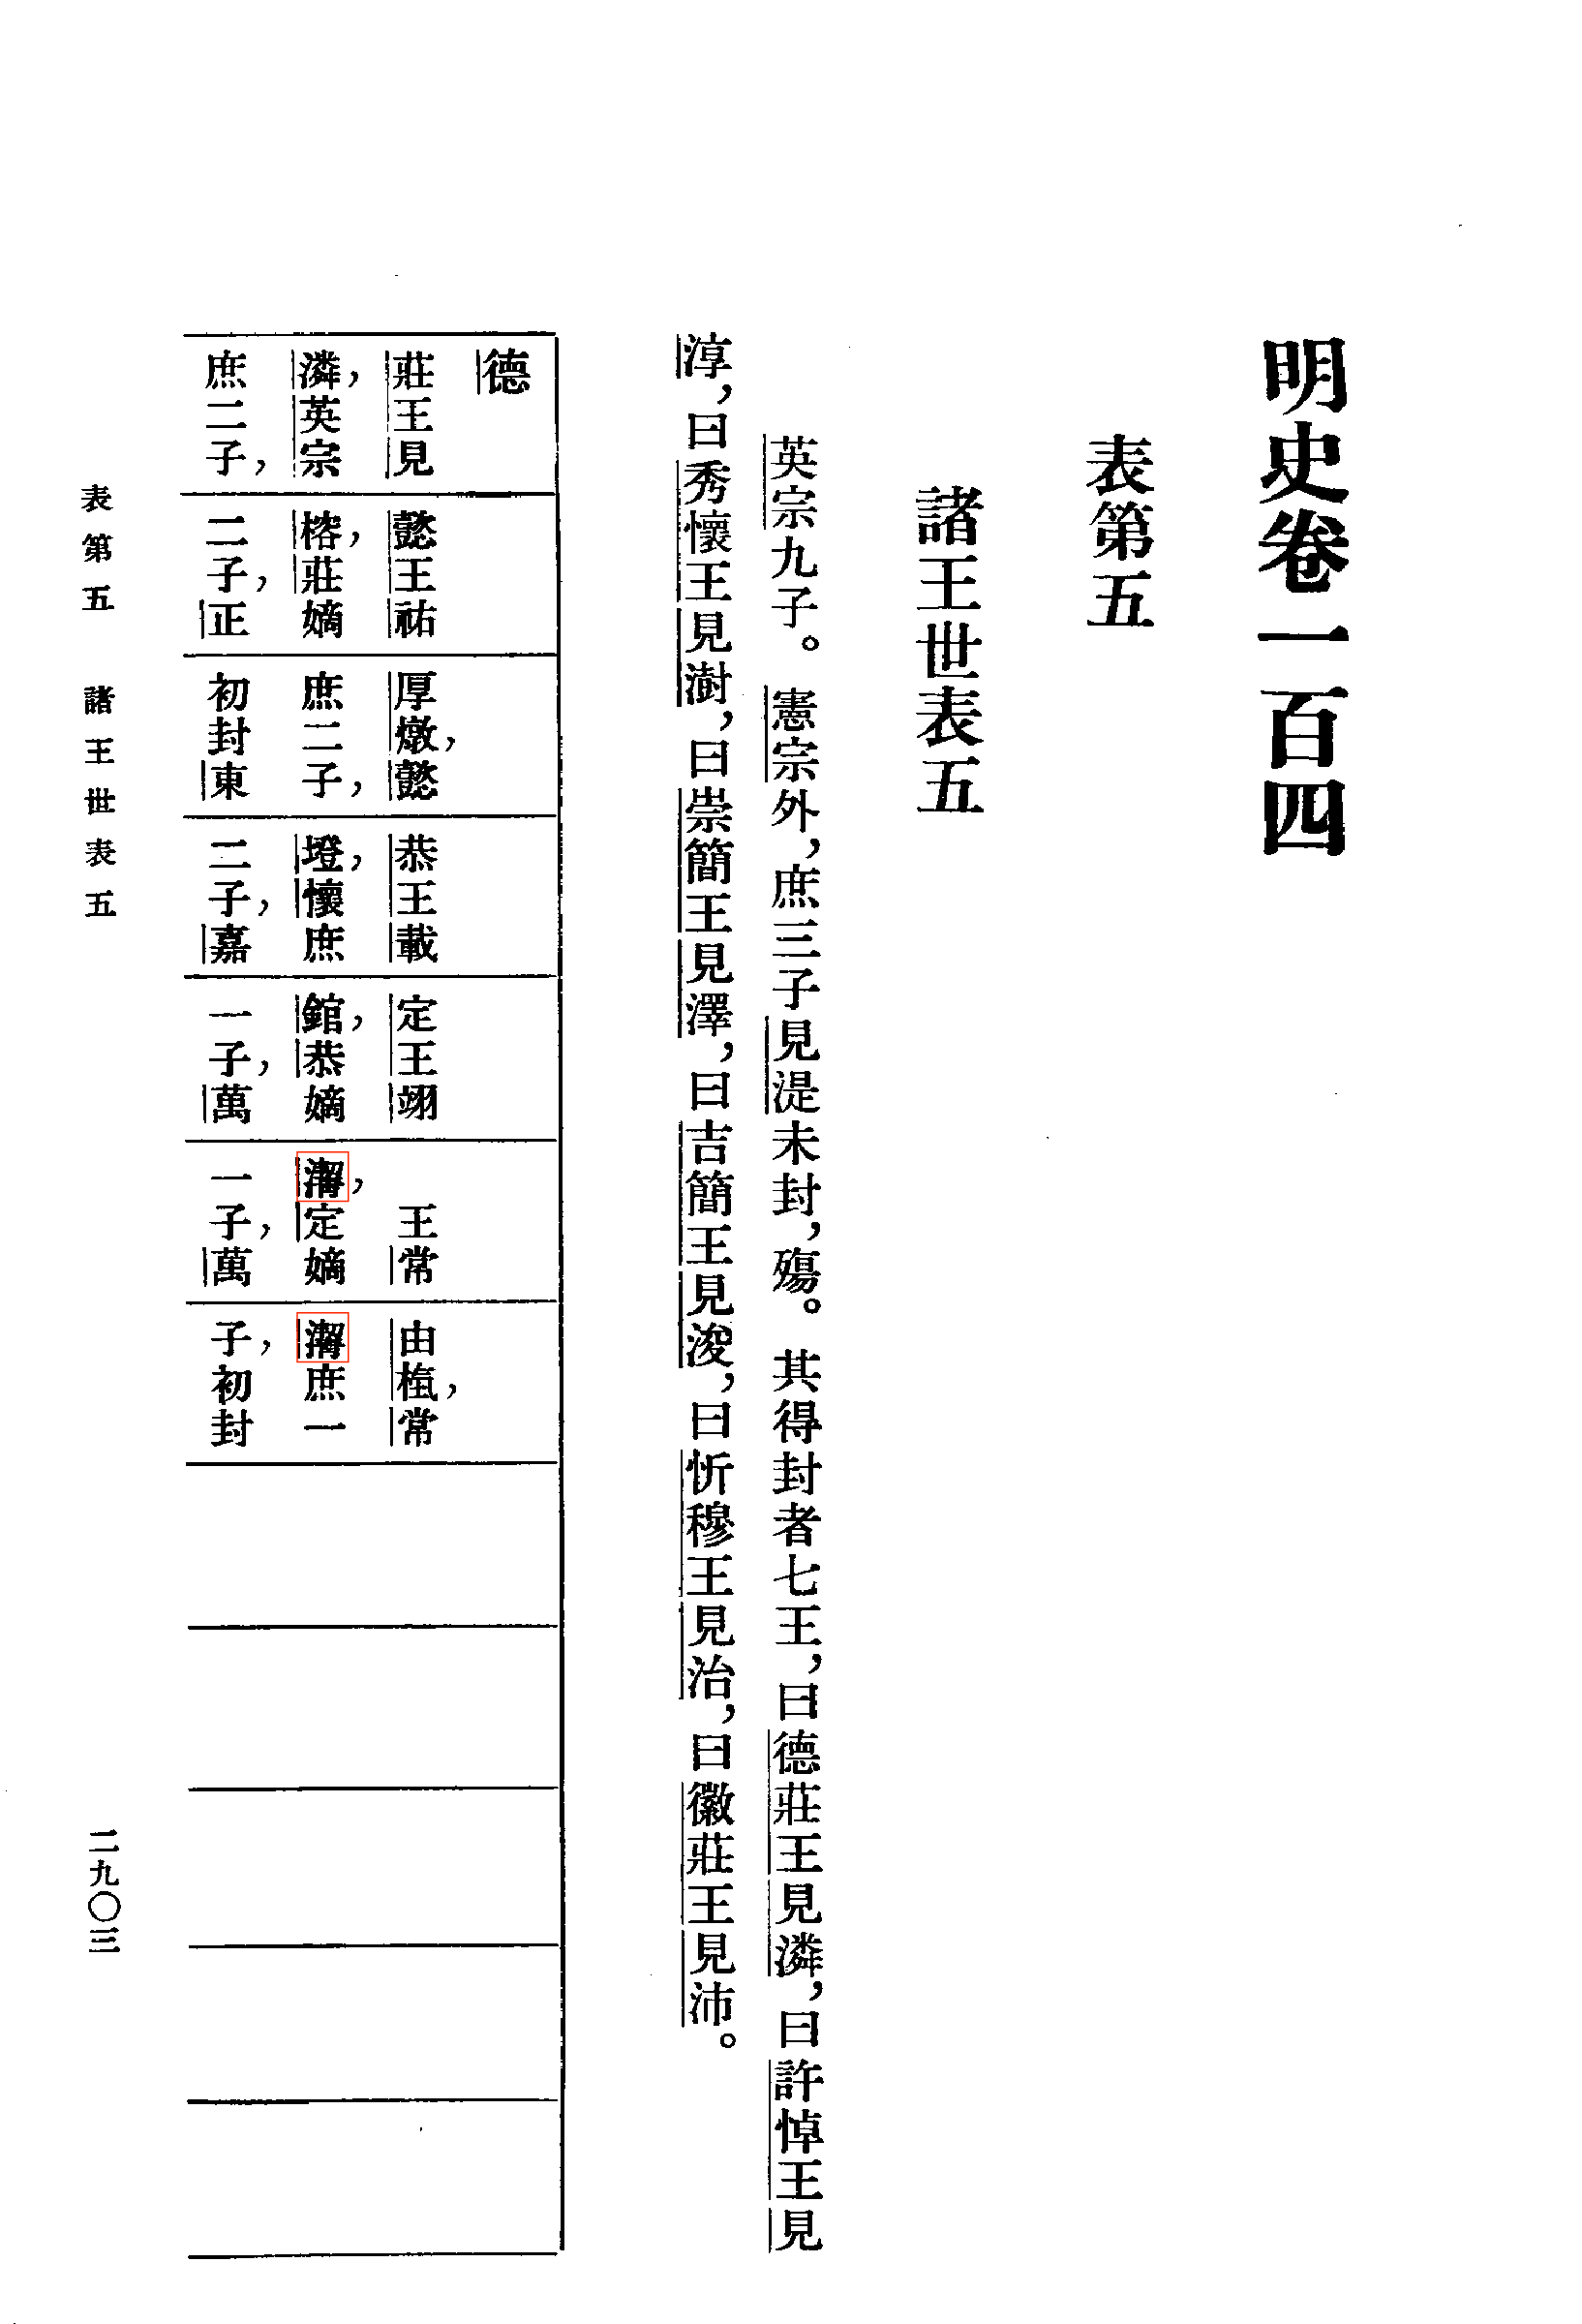
\includegraphics[height=.8\textheight]{002.png} & 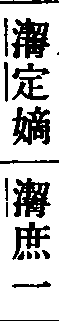
\includegraphics[]{002-crop.png}
    \end{tabular}
    \captionof{figure}{明史(1974,中华书局)page 2903}\label{mingshi1974}
\end{center}

Note that 《南明史》 was authored before 1968 so 錢海岳 has not ever seen 明史(1974,中华书局). The editors of 明史(1974,中华书局)also did not see 南明史 because 錢's manuscript is not found until 1979\cite{南明史}. It is very unusual that both 錢海岳 and experts of 點校本 1) independently changed 﫠 to 𰝙 without supporting evidences from 《明實錄》 and 《明史稿》 2) did not mention why they changed the glyphs.

I suspect 﫠 was replaced by typographers of 中华书局. They might misidentify the 阝 as 刀 and then reordered 氵 to become 𰝙, or they might create the type 𰝙 from 潔 because of reduced efforts. It is not mere speculation as 徐俊, the executive director of 中华书局, mentioned \cite{徐俊谈点校本二十四史的修订} technical challenges in 《宋史·宗室世系表》, which might extend to 《明史·宗室世系表》as well.

\begin{quotation}
    有些问题是纯粹技术原因造成的。《宋史》宗室世系表有很多人名,这些宗室人名用字都是生造的,很多人在史书上没有任何事迹记载,名字只见于宗室表一次。当时铅字排版印刷,如果造字的话,刻字的工作量特别大,所以宗室表里比较后的人名都是用其他字代替的,没有用原字。

    (Translation)
    
    Some of the problems are due to purely technical reasons. There are many person names in the Songshi Imperial Lineage Table, and the characters used for these names are all made up, and many of them have no other records in historical documents, and their names appear only once in the Imperial Lineage Table. At that time, the workload of engraving characters was particularly heavy if all these characters were made, so the names of the people in the later parts of Imperial Lineage Table table were replaced by other characters, and the original characters were not used.
\end{quotation}

After all, 﫠 is reasonable given that 朱常﫠 has a brother named 朱常𰍠\cite{明史德王府世系表訂誤}.

\section{Conclusion}

Based on current evidences, I think 𰝙 is misprint of 﫠. Given that 𰝙 was just encoded in 2020 and 𰝙 is a rare character, either of the following actions should be taken:

1. Add ad-hoc unification for 﫠 and 𰝙, change the reference glyph of U+30759 to 﫠. 

2. Encode 﫠 separately

\bibliography{main}{}
\bibliographystyle{IEEEtran}

\vfill
(End of Document)

\end{document}